\begin{figure*}[!t] \centering
  \begin{tabular}{ccc}
    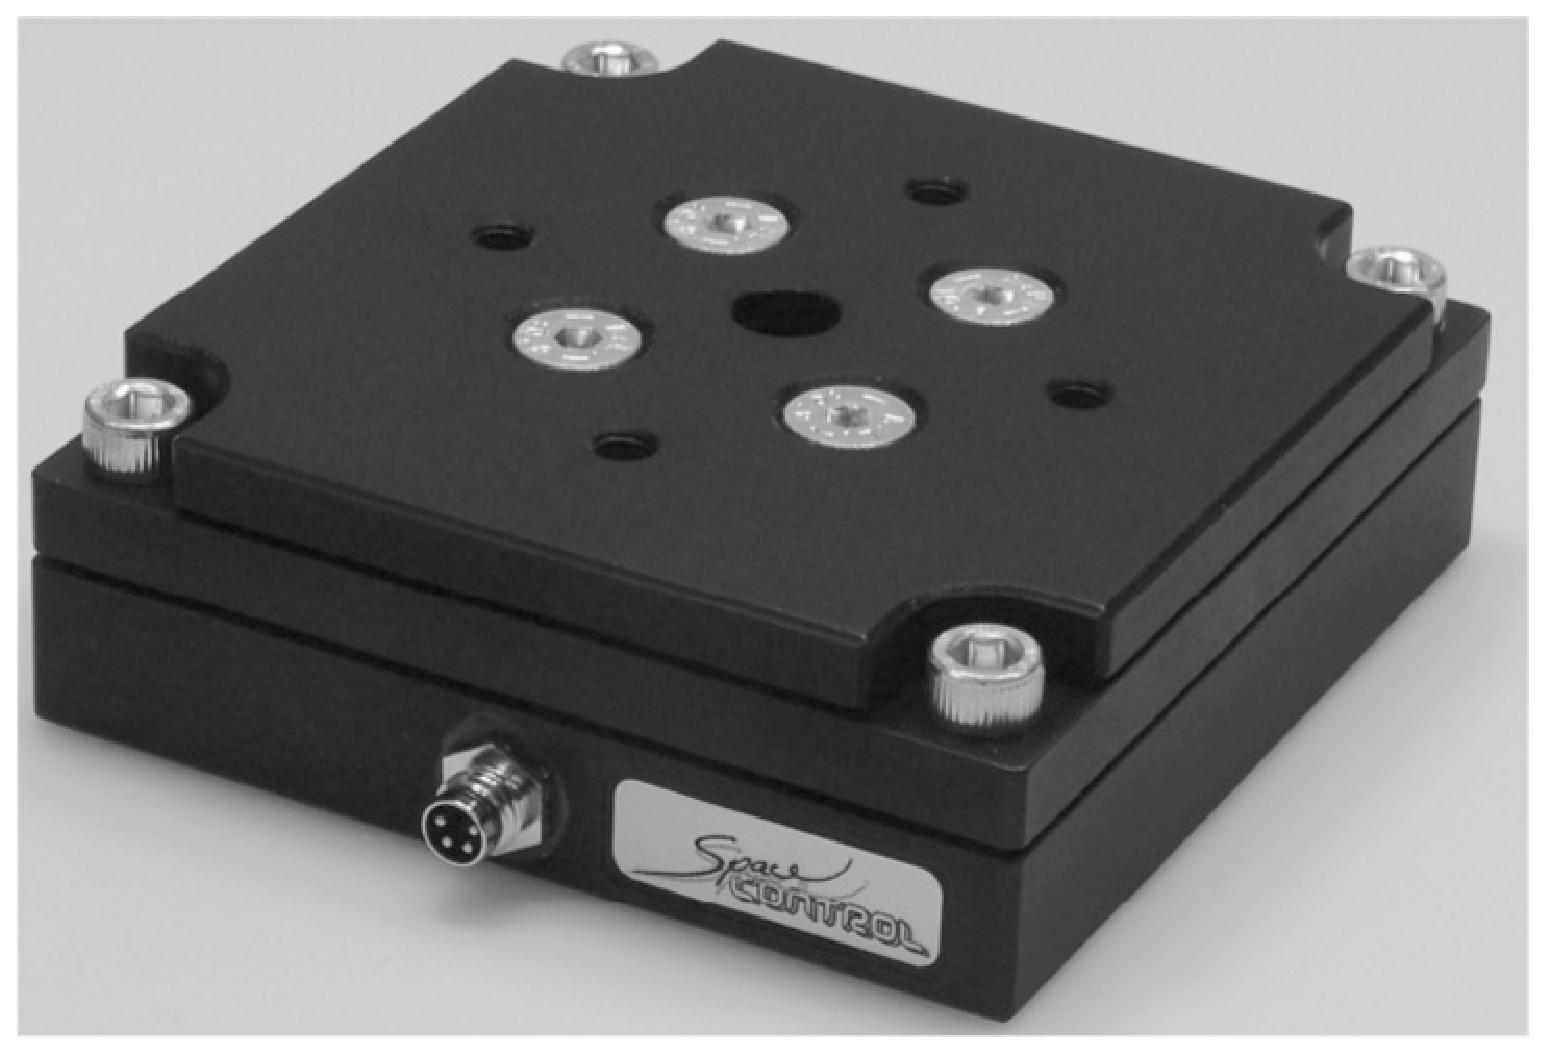
\includegraphics[height=0.16\textheight]{figs/OFTS} &
    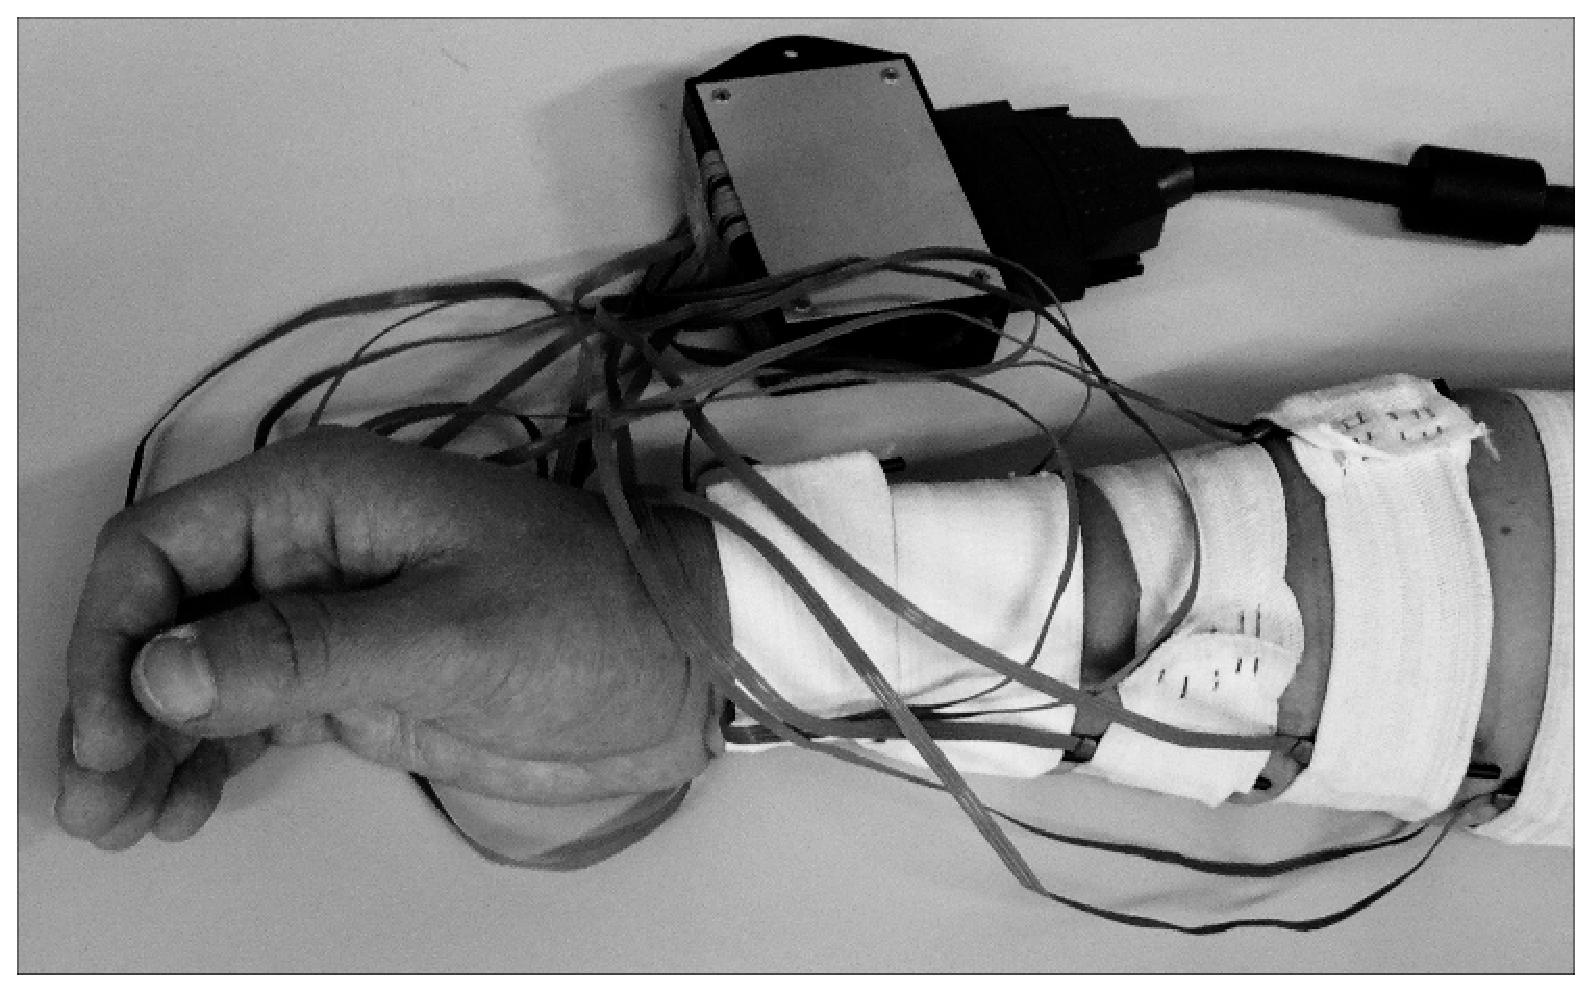
\includegraphics[height=0.16\textheight]{figs/setup} &
    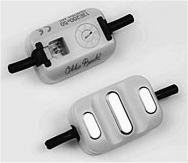
\includegraphics[height=0.16\textheight]{figs/ottobock} \\
    $(a)$ & $(b)$ & $(c)$ \\
  \end{tabular}
  \caption{The experimental setup. (a) The SpaceControl OFTS
    force/torque sensor, large face up. (b)
    The arm of the subject with the EMG electrodes fitted and held in
    place by elastic bands. Electrode cables are wired in a box and
    then directed to a National Instruments PCI-6023E analogic/digital
    conversion card (not shown). (c) An Otto Bock 13E200=50
    surface EMG electrode, with the amplification gauge (upper part of
    the Figure) and the three metallic contacts (lower part).}
  \label{fig:setup}
\end{figure*}

\subsubsection{General setup description}

The experiment consisted of freely, repeatedly grasping a SpaceControl
OFTS force/torque sensor \cite{ofts} orthogonally to its large face
(see Figure~\ref{fig:setup} (a)). Four different ways of pressing
were allowed: opposing the thumb and index, the thumb and middle, the
thumb and ring or the thumb and all other fingers. The speed and force
was intentionally left to the subject's will. Four force sensing
resistors (FSRs) were applied on the subject's hand fingertips (thumb,
index, middle, and ring), in order to be able to detect which grasp
type was used at each instant of time. At the same time, $10$ forearm
surface EMG electrodes were applied to the subject's forearm, held in
place by elastic bands, in order to gather information about the
muscle activation (see Figure \ref{fig:setup} (b)).

Numerical data from the EMG electrodes, FSRs and OFTS were gathered at
the fastest sampling rate we could obtain, that is, $256$Hz, using a
National Instruments DAQ PCI-6023E analog/digital conversion card
\cite{nidaq}, mounted on a fast PC equipped with Windows XP.

\subsubsection{EMG signal and electrode placement}
\label{subsubsec:electrodes}

The $10$ EMG electrodes were applied to the subject's right forearm,
held in place by elastic bands. The electrodes were
double-differential Otto Bock 13E200=50 models (\cite{ottobock}, see
Figure \ref{fig:setup} (c)), each one gifted with an amplification
gauge ranging from $2000$ to $100,000$ times. Initial qualitative
experiments revealed that a safe setting for the amplification gauge
was in the middle of the range, corresponding to about $14,000$
times. This is in agreement with the EMG signal amplitude predicted in
the related literature (see, e.g., \cite{deluca}), that is about $100
\mu$V on average: the voltages our DAQ card read ranged from 0V to
about 2.5V.

Six of the electrodes were placed in pairs along the lower face of the
forearm, whereas four of them were applied in pairs on the upper
face. The initial positioning of the electrodes was chosen in order
for them to lie approximately on top of the muscles which elicit
finger movements; the precise placement was done following the
description in \cite{smagt}, which proved to be optimal for Support
Vector Machine classification of hand postures.

As far as the EMG signal is concerned, it must be remarked that it is
subject to remarkable changes depending on, at least, four orders of
factors:
\begin{enumerate}

  \item \emph{inter-subject variability.} All forearms are different
    from one another in shape, size and power.

  \item \emph{arm posture.} Besides finger movements and grasping, the
    forearm muscles are also involved in the motion of the arm. The
    EMG signal is therefore likely to change if the forearm is moved
    during signal acquisition, for example when switching from
    pronation to supination, or simply while walking around. Even
    raising the shoulder to lift the forearm from the table will
    result in remarkable signal changes.

  \item \emph{electrode displacement.} The intensity and quality of
    the EMG signal depends upon a correct placement of the electrode
    over a muscle. In principle, each electrode should be placed over
    a single muscle, precisely on top of the muscle belly, halfway the
    length of the muscle, and always exactly in the same place.
    Displacing the electrodes will alter the signal, and beside that,
    a precise placement is essentially impossible when dealing with
    surface forearm EMG.

  \item \emph{muscle fatigue.} As the muscles are used more and more,
    continually, fatigue changes the RMS of the EMG signal, calling
    for continual adaptation, at least over a reasonable set of
    different fatigue conditions.

\end{enumerate}

Problems $1$ and $2$ have been for now neglected by concentrating on
one subject only, male, aged $35$ and fully able-bodied, instructed to
keep the arm still and relaxed on a table in a comfortable position,
with the palm orthogonal to the plane of the table. See the Discussion
Section for more about these issues.

As far as muscle fatigue and electrode displacement are concerned,
electrodes \emph{cannot} be expected to exactly lie in the very same
position every time the prosthesis is used; moreover, in a preliminary
round of experiments, muscle fatigue was clearly perceived by the
subject during the experiment. In this framework, the only possibility
to overcome these problems is to explicitly take them into account,
gathering enough data to be able to train the machine under different
conditions of electrode displacement and muscular fatigue.

We then organised the experiment as follows: the subject was
instructed to continuously grasp the sensor over a period of time of
three to four minutes; then he was allowed to rest for about two
minutes. This was called a \emph{session}. It was expected that muscle
fatigue would appear already during one session. Three sessions were
gathered without taking the elastic bands off the subject's forearm,
in order \emph{not} to have electrode displacement within such a set
of sessions, that we called a \emph{group}. After each group, the
electrodes and bands were removed and the subject was allowed for a
much longer period of rest, ranging from half an hour to one
hour. During resting in-between groups, the subject could get back to
his normal muscular activity.

Five groups were then gathered during one day; and this entire
procedure was repeated during another day. This procedure would allow
us to examine a relevant amount of data, gathered along a relatively
long period of time and under different conditions of muscle fatigue
(within one session) and electrode displacement (between
groups). Spectral analysis of the EMG signal revelaed that all
relevant information is limited to $10$Hz (damping of $-30$dB at that
frequency), therefore sampling at $256$Hz proved to be a large
overshoot. We will employ this fact later on.

\subsubsection{Force applied during the grasp}

The OFTS force/torque sensor would output a (negative) integer
numerical value ranging from $0$ to about $-5000$, expressed in
(negative) fiftieths of a Newton. After normalisation, the range of
the applied force would then be between 0N and 100N, with a
resolution of $0.02$N. Linearity of the sensor is guaranteed, and was
anyway manually verified.

\subsubsection{Type of grasp}

The voltage values output by the $4$ FSRs applied onto the subject's
fingertips were monitored in order to understand which kind of grasp
the subject was applying to the sensor. A threshold was experimentally
decided, above which the finger would be defined \emph{in contact}
with the sensor. Using this technique, for each instant in time one of
five possible categories was established: $0$, no action; $1$, grasp
by opposing the thumb and index finger; $2$, opposing thumb and
middle; $3$ thumb and ring; and lastly $4$, grasp by opposing the
thumb and all other fingers.

It must be remarked here that the EMG signal would be altered
immediately at the onset of finger movement, which our setup was
unable to detect. This would result in potentially wrong EMG values for
category $0$. Moreover, the FSRs have been experimentally determined
to suffer from a remarkable hysteresis effect, that is, they will
indicate slightly different voltage while pressing and releasing; this
is due to small rubber ends glued on top of the sensor surfaces, which
aid grasping by raising the static friction coefficient. Hysteresis is
also supposed to somehow degrade the quality of the learning. Because
of these factors we would never expected a close-to-$100\%$
classification accuracy, nor a perfect reconstruction of the applied
force. A better setup is currently being studied, which would avoid
these effects. Again, see the Discussion for more about this issue.
